\section{First tests}

To make this test a list of file is generated, one per DATADISK found in the grid. This list contains only \textit{NTUP\_COMMON}, \textit{NTUP\_SWT2} and \textit{NTUP\_HSG2} files. Some datadisks in the grid does't contain any file of this type then there are not reported in WebDAV/http tests.\\

There are two phases of tests:

\begin{itemize}
	\item \textbf{curl test}: The command tests if the listed file are found on their corresponding disk. Then this tests if the rucio redirection is working, if the site is online, if the disk where is the file is good and it returns an error if failed with the corresponding http code. If this test fails the second one in canceled.
	\item \textbf{davix test}: A C++ compiled program tries to open the file using the Davix library, if this works it tries to read all the events of the branch \textit{el\_n} from the tree \textit{physics}
\end{itemize}

The date of the test is given because WebDAV access is moving a lot over the grid so it's important to report the moment when the test is done in case of just after or during the test there is some configuration modification to corresponding (e.g dCache ugrading, dpm disks crashing or restored...)\\

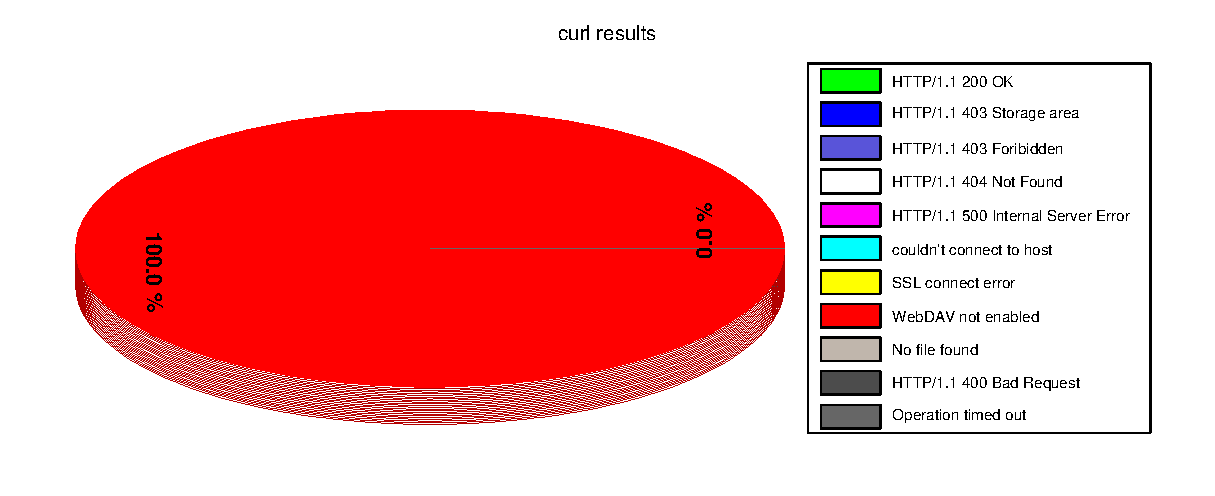
\includegraphics[width=\textwidth]{curlPiecanvas.eps}
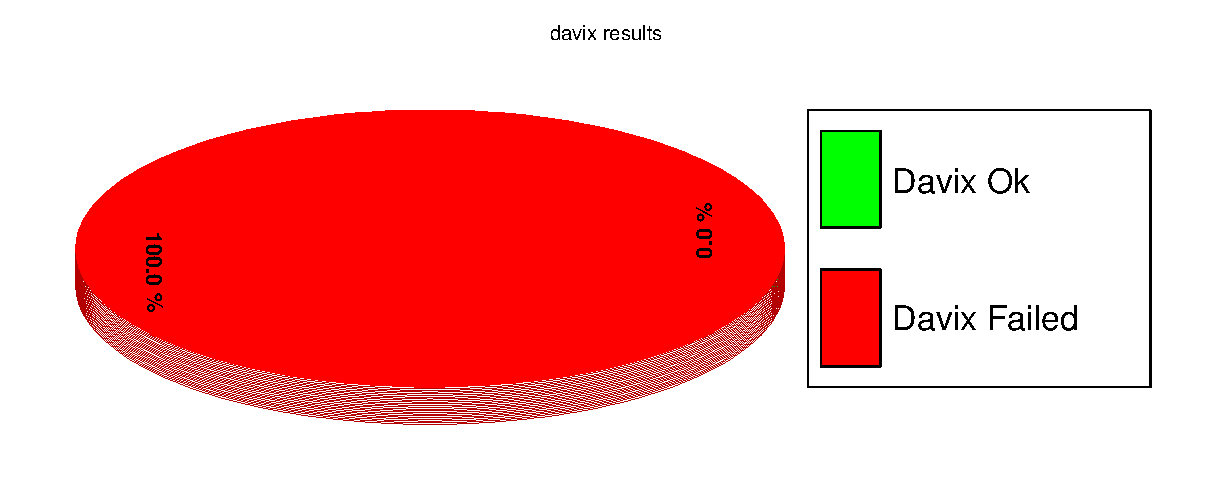
\includegraphics[width=\textwidth]{davixPiecanvas.eps}
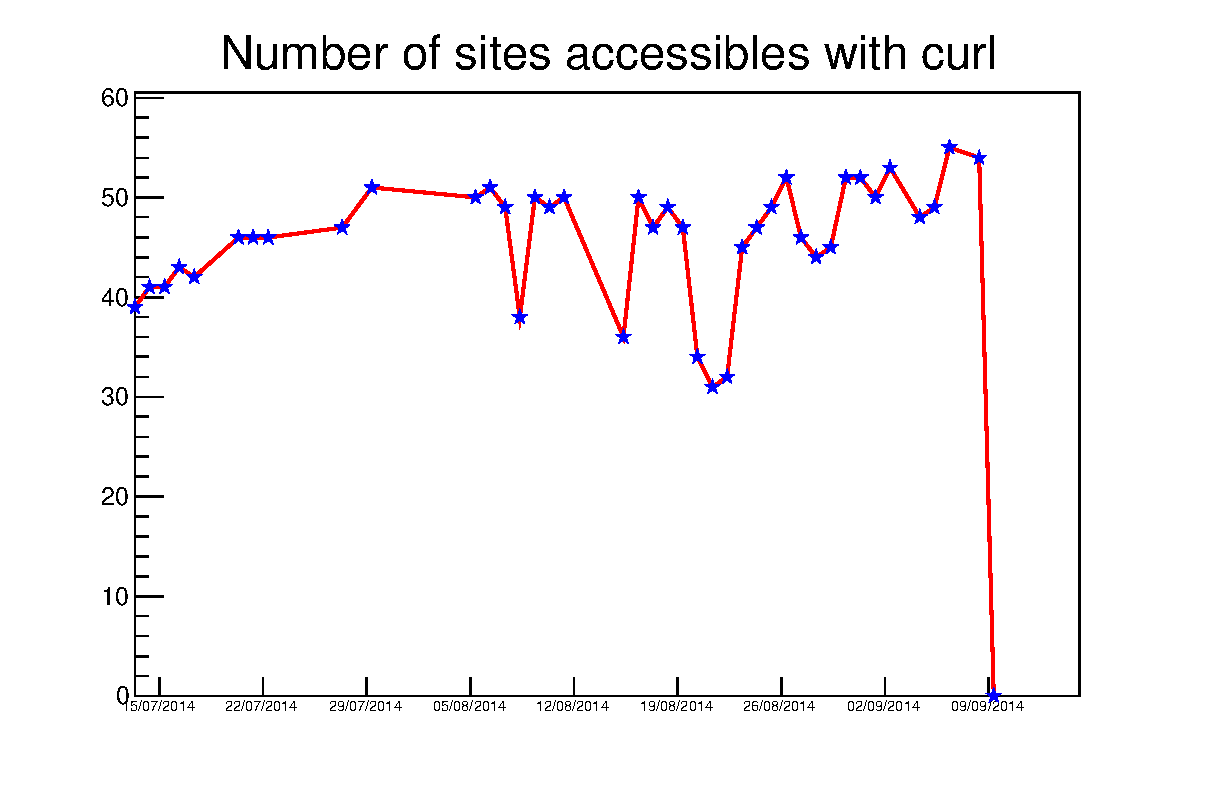
\includegraphics[width=\textwidth]{timeEvolutioncanvas.eps}

